\documentclass[aspectratio=169, 11pt]{beamer}

% ── Theme & colours ──────────────────────────────────────────────
\usetheme{Madrid}
\usecolortheme{seahorse}
\setbeamertemplate{navigation symbols}{}
\setbeamertemplate{footline}[frame number]
\setbeamertemplate{itemize items}[circle]

% ── Packages ─────────────────────────────────────────────────────
\usepackage{amsmath,amssymb}
\usepackage{graphicx}
\usepackage{booktabs}
\usepackage{xcolor}
\usepackage{colortbl}
\usepackage{tikz}
\usetikzlibrary{arrows.meta, positioning, shapes.geometric}

% ── Macros ───────────────────────────────────────────────────────
\newcommand{\bh}{black hole}
\newcommand{\BH}{Black Hole}
\newcommand{\pinn}{PINN}
\newcommand{\pinns}{PINNs}
\newcommand{\qnm}{QNM}
\newcommand{\qnms}{QNMs}
\newcommand{\fd}{FD}
\newcommand{\rw}{Regge--Wheeler}
\newcommand{\zer}{Zerilli}

\definecolor{darkgreen}{rgb}{0.0, 0.5, 0.0}
\definecolor{darkred}{rgb}{0.7, 0.0, 0.0}

% ── Title ────────────────────────────────────────────────────────
\title[QNMs with PINNs]{Computing Quasi-Normal Modes of\\Schwarzschild Black Holes\\with Physics-Informed Neural Networks}
\subtitle{Supervisor Progress Presentation}
\author{Jonathan Chung}
\institute{University of Cambridge}
\date{25 February 2026}

\begin{document}

% ══════════════════════════════════════════════════════════════════
%  TITLE
% ══════════════════════════════════════════════════════════════════
\begin{frame}
  \titlepage
\end{frame}

% ══════════════════════════════════════════════════════════════════
%  OUTLINE
% ══════════════════════════════════════════════════════════════════
\begin{frame}{Outline}
  \tableofcontents
\end{frame}

% ══════════════════════════════════════════════════════════════════
%  SECTION 1 — THE PHYSICS
% ══════════════════════════════════════════════════════════════════
\section{Black Hole Ringdown \& the Master Equation}

% --- Slide 1.1: Motivation ---
\begin{frame}{What Are Quasi-Normal Modes?}
  \begin{itemize}
    \item A perturbed Schwarzschild \bh{} emits gravitational radiation as it settles down --- the \textbf{ringdown}.
    \item The ringdown consists of \textbf{quasi-normal modes} (\qnms{}): damped sinusoids
      \[
        \Phi(t) \propto e^{-t/\tau}\cos(\omega t)
      \]
    \item The frequency $\omega$ and decay time $\tau$ depend \textbf{only on the \bh{} mass} $M$ (for Schwarzschild).
    \item \textbf{Goal:} Solve the perturbation equations numerically to extract $\omega$ and $\tau$.
  \end{itemize}
\end{frame}

% --- Slide 1.2: From Einstein to a 1+1D wave equation ---
\begin{frame}{From Einstein's Equations to a Master Equation}
  Start with the Schwarzschild metric and add a small perturbation:
  \[
    g_{\mu\nu} = g^{0}_{\mu\nu}\text{(Schwarzschild)} + h_{\mu\nu}\text{(small)}
  \]

  \textbf{Key simplifications:}
  \begin{enumerate}
    \item Linearise Einstein's equations in $h_{\mu\nu}$.
    \item Decompose $h_{\mu\nu}$ in \textbf{tensor spherical harmonics} --- angular dependence separates.
    \item Construct a gauge-invariant \textbf{master function} $\Phi$ from the metric perturbation components.
  \end{enumerate}

  \medskip
  Result: a single 1+1D wave equation for each angular mode $\ell$:
  \[
    \boxed{-\frac{\partial^2\Phi}{\partial t^2}
    + \frac{\partial^2\Phi}{\partial x^2}
    - V(r)\,\Phi = 0}
  \]
  where $x = r + 2M\ln\!\bigl(\tfrac{r}{2M}-1\bigr)$ is the \textbf{tortoise coordinate}.
\end{frame}

% --- Slide 1.3: The potentials ---
\begin{frame}{The Potentials}
  The potential $V(r)$ depends on the \textbf{parity} of the perturbation:

  \medskip
  \textbf{Odd-parity (axial) --- \rw{}:}
  \[
    V_{\text{RW}} = \left(1-\frac{2M}{r}\right)\!\left[\frac{\ell(\ell+1)}{r^2} - \frac{6M}{r^3}\right]
  \]

  \textbf{Even-parity (polar) --- \zer{}:}
  \[
    V_{\text{Z}} = \left(1-\frac{2M}{r}\right)\frac{2n^2(n+1)r^3 + 6n^2Mr^2 + 18nM^2r + 18M^3}{r^3(nr+3M)^2}
  \]
  where $2n = (\ell-1)(\ell+2)$.

  \medskip
  \begin{itemize}
    \item Both potentials peak near $x \sim 1M$ and vanish at the horizon and infinity.
    \item A transformation connects them (Chandrasekhar) $\Rightarrow$ \textbf{same \qnms{}}.
    \item We focus on the \textbf{\zer{} potential} with $\ell = 2$ (dominant mode).
  \end{itemize}
\end{frame}

% --- Slide 1.4: BCs and ICs ---
\begin{frame}{Boundary \& Initial Conditions}
  \textbf{Boundary conditions} (Sommerfeld --- radiation conditions):
  \begin{align*}
    \text{Horizon } (x\to -\infty): &\quad \left(\partial_t - \partial_x\right)\Phi = 0 \quad \text{(ingoing)}\\
    \text{Infinity } (x\to +\infty): &\quad \left(\partial_t + \partial_x\right)\Phi = 0 \quad \text{(outgoing)}
  \end{align*}

  \textbf{Initial conditions} --- outgoing Gaussian pulse:
  \begin{align*}
    \Phi(x, 0) &= \exp\!\left[-\frac{(x - 4M)^2}{(5M)^2}\right]\\[4pt]
    \partial_t\Phi(x, 0) &= -\partial_x\Phi(x,0) \quad \text{(purely right-moving)}
  \end{align*}

  \textbf{Domain:} $x/M \in [-50, 150]$, \quad $t/M \in [0, 50]$.

  \medskip
  The pulse scatters off the potential barrier $\;\Rightarrow\;$ ringdown at late times.
\end{frame}

% --- Slide 1.5: 3D Waveform ---
\begin{frame}{Ringdown Waveform --- 3D Visualisation}
  \begin{center}
    \includegraphics[width=0.85\textwidth,height=0.82\textheight,keepaspectratio]{../outputs/pinn/zerilli_l2_rad_k2/waveform_3d.png}
  \end{center}
\end{frame}


% ══════════════════════════════════════════════════════════════════
%  SECTION 2 — THE METHOD
% ══════════════════════════════════════════════════════════════════
\section{Methodology: PINNs \& Finite Differences}

% --- Slide 2.1: PINN concept ---
\begin{frame}{Physics-Informed Neural Networks --- Core Idea}
  Instead of a grid, train a neural network $\Phi_{\boldsymbol{\theta}}(x,t)$
  to satisfy the PDE, BCs, and ICs simultaneously.

  \vspace{0.3cm}
  \begin{center}
  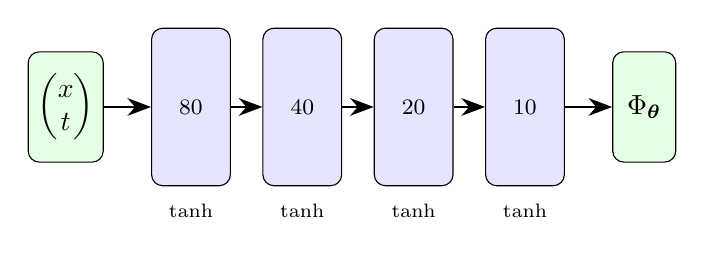
\begin{tikzpicture}[
      node distance=1.2cm,
      layer/.style={draw, rounded corners, minimum width=1.0cm, minimum height=2.0cm, fill=blue!10},
      io/.style={draw, rounded corners, minimum width=0.8cm, minimum height=1.4cm, fill=green!10},
      arr/.style={-{Stealth[length=3mm]}, thick}
    ]
    \node[io] (input) {$\begin{pmatrix}x\\t\end{pmatrix}$};
    \node[layer, right=0.6cm of input] (h1) {\footnotesize 80};
    \node[layer, right=0.4cm of h1] (h2) {\footnotesize 40};
    \node[layer, right=0.4cm of h2] (h3) {\footnotesize 20};
    \node[layer, right=0.4cm of h3] (h4) {\footnotesize 10};
    \node[io, right=0.6cm of h4] (output) {$\Phi_{\boldsymbol{\theta}}$};

    \draw[arr] (input) -- (h1);
    \draw[arr] (h1) -- (h2);
    \draw[arr] (h2) -- (h3);
    \draw[arr] (h3) -- (h4);
    \draw[arr] (h4) -- (output);

    \node[below=0.1cm of h1, font=\scriptsize] {tanh};
    \node[below=0.1cm of h2, font=\scriptsize] {tanh};
    \node[below=0.1cm of h3, font=\scriptsize] {tanh};
    \node[below=0.1cm of h4, font=\scriptsize] {tanh};
  \end{tikzpicture}
  \end{center}
  \vspace{0.1cm}

  \begin{itemize}
    \item 4 hidden layers, $\tanh$ activation, Glorot uniform initialisation.
    \item Output transform: $\Phi_{\boldsymbol{\theta}} = A\tanh(\text{raw output})$ bounds the solution to $[-1,1]$.
    \item Derivatives via \textbf{automatic differentiation} (exact, no discretisation error).
    \item \textbf{4,521 trainable parameters.}
  \end{itemize}
\end{frame}

% --- Slide 2.2: Loss function ---
\begin{frame}{The Loss Function}
  Train by minimising a weighted sum of 7 terms:
  \[
    \mathcal{L} = \boldsymbol{\lambda}\cdot\bigl[\,
      \underbrace{\mathcal{L}_r,\;\mathcal{L}_{r_x},\;\mathcal{L}_{r_t}}_{\text{PDE residual}},\;
      \underbrace{\mathcal{L}_{ic},\;\mathcal{L}_{iv}}_{\text{initial conds.}},\;
      \underbrace{\mathcal{L}_{bl},\;\mathcal{L}_{br}}_{\text{boundary conds.}}
    \,\bigr]
  \]

  \medskip
  \begin{tabular}{@{}lll@{}}
    \toprule
    \textbf{Term} & \textbf{Penalises} & \textbf{Points} \\
    \midrule
    $\mathcal{L}_r$ & $\Phi_{tt} - \Phi_{xx} + V\Phi \neq 0$ & $N_r = 32{,}000$ \\
    $\mathcal{L}_{r_x},\,\mathcal{L}_{r_t}$ & Gradients of residual (gradient-enhanced \pinn{}) & same \\
    $\mathcal{L}_{ic},\,\mathcal{L}_{iv}$ & Initial profile \& velocity mismatch & $N_i = 800$ \\
    $\mathcal{L}_{bl},\,\mathcal{L}_{br}$ & Sommerfeld BC violations & $N_b = 400$ \\
    \bottomrule
  \end{tabular}

  \medskip
  \begin{itemize}
    \item \textbf{Phase problem:} $\Phi(x, t+\alpha)$ is also a solution $\Rightarrow$ weight $\lambda_{iv}$ heavily to lock the correct phase.
    \item Total: \textbf{33,600 collocation points} (vs.\ 500,000 grid points for \fd{}).
  \end{itemize}
\end{frame}

% --- Slide 2.3: Training procedure ---
\begin{frame}{Two-Phase Training}
  \begin{columns}[T]
    \begin{column}{0.48\textwidth}
      \textbf{Phase 1: Adam} (10,000 iters)
      \begin{itemize}
        \item Stochastic gradient descent with adaptive learning rate ($\text{lr}=10^{-3}$).
        \item Good at rough, global exploration.
        \item Uniform point resampling every 100 iters.
      \end{itemize}
    \end{column}
    \begin{column}{0.48\textwidth}
      \textbf{Phase 2: L-BFGS} (15,000 iters)
      \begin{itemize}
        \item Quasi-Newton: approximates inverse Hessian from gradient history.
        \item Fast, precise convergence near minima.
        \item Sensitive to point changes $\Rightarrow$ only uniform resampling here.
      \end{itemize}
    \end{column}
  \end{columns}

  \vspace{0.5cm}
  \begin{center}
    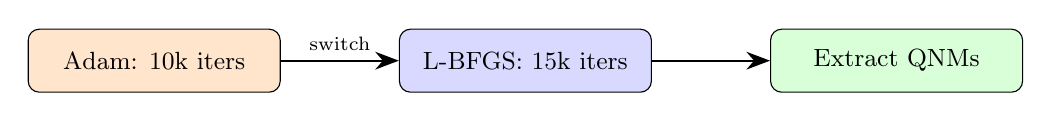
\begin{tikzpicture}[
        box/.style={draw, rounded corners, minimum width=3.2cm, minimum height=0.8cm, font=\small},
        arr/.style={-{Stealth[length=3mm]}, thick}
      ]
      \node[box, fill=orange!20] (adam) {Adam: 10k iters};
      \node[box, fill=blue!15, right=1.5cm of adam] (lbfgs) {L-BFGS: 15k iters};
      \node[box, fill=green!15, right=1.5cm of lbfgs] (done) {Extract \qnms{}};
      \draw[arr] (adam) -- node[above, font=\scriptsize]{switch} (lbfgs);
      \draw[arr] (lbfgs) -- (done);
    \end{tikzpicture}
  \end{center}
\end{frame}

% --- Slide 2.4: FD baseline ---
\begin{frame}{Finite Difference Baseline}
  For comparison, we solve the same PDE with standard numerical methods:
  \begin{itemize}
    \item Uniform mesh: $N_x = 1{,}000$ points, $\Delta x = 0.2M$.
    \item Method of lines + 4th-order Runge--Kutta, $\Delta t = 0.1M$.
    \item 500 time steps $\Rightarrow$ $N_F = 500{,}000$ grid points.
  \end{itemize}

  \medskip
  The \fd{} solution serves as \textbf{ground truth} for evaluating the \pinn{}.

  \medskip
  \textbf{Key comparison:}
  \begin{center}
    \begin{tabular}{@{}lcc@{}}
      \toprule
      & \textbf{\fd{}} & \textbf{\pinn{}} \\
      \midrule
      Representation & Grid values $\Phi_{i,j}$ & Neural network $\Phi_{\boldsymbol{\theta}}(x,t)$ \\
      Derivatives & FD stencils (approx.) & Autograd (exact) \\
      Points & 500,000 & 33,600 \\
      Time-stepping & Explicit RK4 & None (global solve) \\
      \bottomrule
    \end{tabular}
  \end{center}
\end{frame}

% --- Slide 2.5: QNM extraction ---
\begin{frame}{Extracting Quasi-Normal Modes}
  Sample $\Phi(x_q, t)$ at observation point $x_q = 10M$, restrict to late times.

  \medskip
  \textbf{Method 1} --- FFT + Envelope:
  \begin{itemize}
    \item $\omega$: FFT of $\Phi(x_q,t)$ $\;\Rightarrow\;$ peak frequency.
    \item $\tau$: Linear fit to $\ln|\text{envelope peaks}|$ vs.\ $t$ $\;\Rightarrow\;$ slope $= -1/\tau$.
  \end{itemize}

  \textbf{Method 2} --- Direct curve fit:
  \begin{itemize}
    \item Fit $\Phi \approx A\,e^{-t/\tau}\cos(\omega t + \phi)$ directly via nonlinear least squares.
  \end{itemize}

  \medskip
  Compare extracted $(\omega, \tau)$ against theoretical values (Leaver 1985):
  \begin{center}
    \begin{tabular}{@{}ccc@{}}
      \toprule
      $\ell$ & $\omega M$ & $\tau/M$ \\
      \midrule
      2 & 0.3737 & 11.241 \\
      \bottomrule
    \end{tabular}
  \end{center}
\end{frame}


% ══════════════════════════════════════════════════════════════════
%  SECTION 3 — RESULTS
% ══════════════════════════════════════════════════════════════════
\section{Results}

% --- Slide 3.1: Paper reproduction ---
\begin{frame}{Paper Reproduction: Baseline Results}
  Reproduced the setup of Patel, Aykutalp \& Laguna (2024) with our corrected
  outgoing initial velocity profile.

  \begin{columns}[T]
    \begin{column}{0.52\textwidth}
      \begin{center}
        % ── Suggested plot: snapshots or ringdown_overlay from paper repro ──
        \includegraphics[width=\textwidth]{../../project32_qnm_pinn/outputs/pinn/zerilli_l2_paper/snapshots.png}
        \\{\footnotesize Waveform snapshots: \pinn{} vs.\ \fd{} (uniform sampling)}
      \end{center}
    \end{column}
    \begin{column}{0.45\textwidth}
      {\small Zerilli $\ell=2$ QNM Extraction}

      \smallskip
      \begin{tabular}{@{}lcc@{}}
        \toprule
        & $\boldsymbol{\tau/M}$ & $\boldsymbol{\omega M}$ \\
        \midrule
        \textbf{TRUE}     & 11.241 & 0.3737  \\
        \midrule
        \textbf{FD$_1$}   & 10.929\,{\scriptsize(2.78)} & 0.3716\,{\scriptsize(0.56)}  \\
        \textbf{FD$_2$}   & 11.465\,{\scriptsize(2.00)} & 0.3798\,{\scriptsize(1.63)}  \\
        \textbf{PINN$_1$} & 10.671\,{\scriptsize(5.07)} & 0.3697\,{\scriptsize(1.08)}  \\
        \textbf{PINN$_2$} & 11.410\,{\scriptsize(1.50)} & 0.3784\,{\scriptsize(1.25)}  \\
        \bottomrule
      \end{tabular}

      \smallskip
      {\scriptsize Parentheses: \% error vs.\ Leaver 1985.\\[2pt]
      Subscript 1 = FFT + envelope.\\[1pt]
      Subscript 2 = direct curve fit.}
    \end{column}
  \end{columns}
\end{frame}

% --- Slide 3.2: Curve fitting (paper repro) ---
\begin{frame}{Curve Fitting --- Paper Reproduction}
  \begin{center}
    \includegraphics[width=0.75\textwidth,height=0.78\textheight,keepaspectratio]{../../project32_qnm_pinn/outputs/pinn/zerilli_l2_paper/curve_fitting.png}
  \end{center}
  \vspace{-0.2cm}
  \small
  $\log|\Phi|$ vs.\ $t/M$ at $x_q = 10M$. All five reconstructed damped cosines
  $A\,e^{-t/\tau}\cos(\omega t + \phi)$ overlap closely --- both FD and PINN
  extract QNMs within $\sim$1--4\% of the Leaver (1985) values.
\end{frame}

% --- Slide 3.2b: Accuracy comparison vs paper ---
\begin{frame}{QNM Accuracy: Our Results vs.\ the Paper}
  \begin{center}
    {\small Zerilli $\ell = 2$ --- $\tau/M$ and $\omega M$ percentage errors}

    \medskip
    \begin{tabular}{@{}l cc c cc@{}}
      \toprule
      & \multicolumn{2}{c}{\textbf{Paper} (Patel et al.)} && \multicolumn{2}{c}{\textbf{Ours}} \\
      \cmidrule{2-3} \cmidrule{5-6}
      & $\tau/M$ \,(\% err) & $\omega M$ \,(\% err) && $\tau/M$ \,(\% err) & $\omega M$ \,(\% err) \\
      \midrule
      \textbf{FD$_1$}   & 10.804\;(3.89) & 0.370\;(0.90) && 10.929\;(2.78) & 0.372\;(0.56) \\
      \textbf{FD$_2$}   & 11.073\;(1.49) & 0.378\;(1.26) && 11.465\;(2.00) & 0.380\;(1.63) \\
      \textbf{PINN$_1$} & 10.089\;(10.25) & 0.375\;(0.29) && 10.671\;(\textbf{5.07}) & 0.370\;(1.08) \\
      \textbf{PINN$_2$} & \textcolor{darkred}{9.620\;(14.42)} & 0.376\;(0.52) && \textcolor{darkgreen}{11.410\;(\textbf{1.50})} & 0.378\;(1.25) \\
      \bottomrule
    \end{tabular}
  \end{center}

  \bigskip
  \begin{itemize}
    \item \textbf{Major improvement:} PINN$_2$ decay time error drops from
          \textcolor{darkred}{14.42\%} $\;\to\;$ \textcolor{darkgreen}{1.50\%}
          ($\mathbf{9.6\times}$ more accurate).
    \item PINN$_1$ $\tau$ error also improves: $10.25\% \to 5.07\%$ ($2.0\times$).
    \item Likely cause: our corrected outgoing initial velocity
          $\partial_t\Phi = -\partial_x\Phi$ (Sommerfeld condition).
  \end{itemize}
\end{frame}

% --- Slide 3.3: RAD explained ---
\begin{frame}{Our Improvement: Residual-Adaptive Distribution (RAD)}
  \textbf{Problem:} Uniform sampling wastes points in empty regions where $\Phi \approx 0$.

  \medskip
  \textbf{RAD} (Wu et al.\ 2023): Every $P$ training steps during Adam---
  \begin{enumerate}
    \item Generate 100,000 random candidate points.
    \item Evaluate PDE residual $|r_i|$ at each candidate.
    \item Compute sampling probability: $\displaystyle p_i \propto |r_i|^k + c$.
    \item Sample 32,000 points from candidates $\Rightarrow$ replace all domain points.
  \end{enumerate}

  \medskip
  \begin{center}
    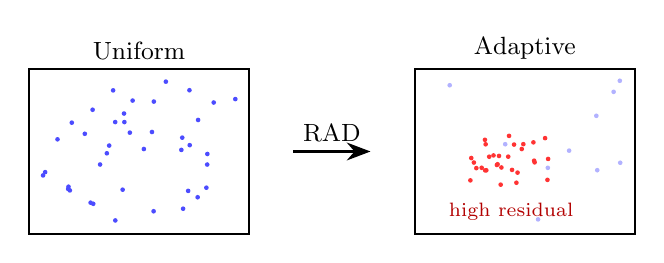
\begin{tikzpicture}[scale=0.7]
      % Uniform
      \draw[thick] (0,0) rectangle (4,3);
      \node[above] at (2,3) {\small Uniform};
      \foreach \i in {1,...,40}{
        \pgfmathsetmacro{\px}{0.2+3.6*rnd}
        \pgfmathsetmacro{\py}{0.2+2.6*rnd}
        \fill[blue!70] (\px,\py) circle (1.2pt);
      }

      % Arrow
      \draw[-{Stealth[length=3mm]}, very thick] (4.8,1.5) -- (6.2,1.5);
      \node[above] at (5.5,1.5) {\small RAD};

      % RAD
      \draw[thick] (7,0) rectangle (11,3);
      \node[above] at (9,3) {\small Adaptive};
      % sparse region
      \foreach \i in {1,...,10}{
        \pgfmathsetmacro{\px}{7.2+3.6*rnd}
        \pgfmathsetmacro{\py}{0.2+2.6*rnd}
        \fill[blue!30] (\px,\py) circle (1.2pt);
      }
      % dense cluster (high residual region)
      \foreach \i in {1,...,30}{
        \pgfmathsetmacro{\px}{8.0+1.5*rnd}
        \pgfmathsetmacro{\py}{0.8+1.0*rnd}
        \fill[red!80] (\px,\py) circle (1.2pt);
      }
      \node[font=\scriptsize, text=darkred] at (8.75,0.4) {high residual};
    \end{tikzpicture}
  \end{center}
\end{frame}

% --- Slide 3.4: RAD tuning results ---
\begin{frame}{RAD Tuning Experiments}
  \begin{center}
    \begin{tabular}{@{}lccccc@{}}
      \toprule
      \textbf{Configuration} & \textbf{$k$} & \textbf{$c$} & \textbf{Final Loss} & \textbf{RMSD} & \textbf{RL2} \\
      \midrule
      Uniform (paper repro) & --- & --- & $1.18\times10^{-6}$ & 0.00183 & 1.30\% \\
      RAD baseline          & 1   & 1   & $7.40\times10^{-7}$ & 0.00115 & 0.82\% \\
      \rowcolor{green!10}
      RAD aggressive         & 2   & 0.1 & $9.07\times10^{-7}$ & \textbf{0.00095} & \textbf{0.67\%} \\
      RAD $k\!=\!2$, $P\!=\!500$ & 2 & 0.1 & $1.06\times10^{-6}$ & 0.00105 & 0.75\% \\
      RAD + anchor (20\%)        & 1 & 1   & $8.20\times10^{-7}$ & 0.00141 & 1.00\% \\
      \bottomrule
    \end{tabular}
  \end{center}

  \medskip
  \begin{itemize}
    \item RAD reduces RMSD by \textbf{37\%} over uniform sampling.
    \item Aggressive RAD ($k\!=\!2$) achieves the \textbf{best RMSD} (0.00095).
    \item Anchor retention has the \textbf{second-lowest loss} ($8.20\times10^{-7}$) but the \textbf{highest RMSD} among RAD runs --- suggests over-fitting to anchor points at the expense of global accuracy.
  \end{itemize}
\end{frame}



% --- Slide 3.6: Error heatmap ---
\begin{frame}{Spatial Error Distribution}
  \begin{columns}[T]
    \begin{column}{0.48\textwidth}
      \begin{center}
        % ── Suggested plot: error heatmap from paper repro ──
        \includegraphics[width=\textwidth]{../../project32_qnm_pinn/outputs/pinn/zerilli_l2_paper/error_heatmap.png}
        \\{\footnotesize Uniform sampling}
      \end{center}
    \end{column}
    \begin{column}{0.48\textwidth}
      \begin{center}
        % ── Suggested plot: error heatmap from RAD ──
        \includegraphics[width=\textwidth]{../outputs/pinn/zerilli_l2_rad/error_heatmap.png}
        \\{\footnotesize RAD adaptive sampling}
      \end{center}
    \end{column}
  \end{columns}

  \medskip
  \begin{center}
    RAD reduces the error concentration at the \textbf{wavefront leading edge}.
  \end{center}
\end{frame}

% --- Slide 3.7: Ringdown overlay ---
\begin{frame}{Ringdown Waveform at $x_q = 10M$}
  \begin{columns}[T]
    \begin{column}{0.48\textwidth}
      \begin{center}
        \includegraphics[width=\textwidth]{../outputs/pinn/zerilli_l2_rad/ringdown_overlay.png}
        \\{\footnotesize RAD baseline: \pinn{} vs.\ \fd{} (raw waveforms)}
      \end{center}
    \end{column}
    \begin{column}{0.48\textwidth}
      \begin{center}
        \includegraphics[width=\textwidth]{../outputs/pinn/zerilli_l2_rad_k2/ringdown_overlay.png}
        \\{\footnotesize RAD $k=2$: \pinn{} vs.\ \fd{} (raw waveforms)}
      \end{center}
    \end{column}
  \end{columns}

  \medskip
  \begin{center}
    Top: linear scale; Bottom: $\log|\Phi|$. Both variants closely match the \fd{} reference.
  \end{center}
\end{frame}

% --- Slide 3.7b: Curve fitting — RAD k=2 ---
\begin{frame}{Curve Fitting --- RAD $k\!=\!2$}
  \begin{columns}[T]
    \begin{column}{0.52\textwidth}
      \begin{center}
        \includegraphics[width=\textwidth]{../outputs/pinn/zerilli_l2_rad_k2/curve_fitting.png}
        \\{\footnotesize $\log|\Phi|$ vs.\ $t/M$ at $x_q = 10M$ (RAD $k\!=\!2$)}
      \end{center}
    \end{column}
    \begin{column}{0.46\textwidth}
      {\small Zerilli $\ell=2$ --- QNM Extraction}

      \smallskip
      \begin{tabular}{@{}lcc@{}}
        \toprule
        & $\boldsymbol{\tau/M}$ & $\boldsymbol{\omega M}$ \\
        \midrule
        \textbf{TRUE}     & 11.241 & 0.3737  \\
        \midrule
        \textbf{FD$_1$}   & 10.929\,{\scriptsize(2.78)} & 0.3716\,{\scriptsize(0.56)}  \\
        \textbf{FD$_2$}   & 11.465\,{\scriptsize(2.00)} & 0.3798\,{\scriptsize(1.63)}  \\
        \textbf{PINN$_1$} & 10.831\,{\scriptsize(3.65)} & 0.3705\,{\scriptsize(0.85)}  \\
        \textbf{PINN$_2$} & 11.443\,{\scriptsize(1.80)} & 0.3790\,{\scriptsize(1.43)}  \\
        \bottomrule
      \end{tabular}

      \smallskip
      {\scriptsize FD$_{1,2}$ identical to paper repro\\(same FD solver).\\[2pt]
      PINN$_{1,2}$ from RAD $k\!=\!2$ run.}
    \end{column}
  \end{columns}

  \medskip
  \begin{itemize}
    \item RAD PINN$_2$: $\tau$ error 1.80\% vs.\ 1.50\% (paper repro) --- comparable accuracy.
    \item RAD primarily improves \textbf{spatial} accuracy (RMSD), not QNM extraction.
  \end{itemize}
\end{frame}

% --- Slide 3.8: Summary ---
\begin{frame}{Summary of Findings}
  \begin{enumerate}
    \item \textbf{PINNs can compute \qnms{}} of Schwarzschild \bh{}s to within $\sim$1--2\% of known values,
          using $15\times$ fewer collocation points than \fd{}.

    \medskip
    \item \textbf{RAD adaptive sampling} improves solution accuracy by $\sim$37\% (RMSD)
          over uniform sampling, by concentrating points where the PDE residual is largest.

    \medskip
    \item \textbf{Aggressive RAD} ($k=2$) provides the best spatial accuracy (lowest RMSD/RL2).
          Anchor retention has the second-lowest loss but the highest RMSD among RAD runs --- over-fitting to anchor points.

    \medskip
    \item \textbf{Exponential reweighting fails} --- naively amplifying late-time residuals
          destabilises training ($\tau$ error $>$20\%).
  \end{enumerate}
\end{frame}

% ══════════════════════════════════════════════════════════════════
%  BACKUP / THANK YOU
% ══════════════════════════════════════════════════════════════════
\begin{frame}{}
  \begin{center}
    {\Large Thank you}

    \bigskip
    Questions?
  \end{center}
\end{frame}

% ══════════════════════════════════════════════════════════════════
%  APPENDIX
% ══════════════════════════════════════════════════════════════════
\appendix

% --- Appendix: Reproduction Run Loss ---
\begin{frame}{Appendix: Loss History --- Reproduction Run (Uniform Sampling)}
  \begin{center}
    \includegraphics[width=0.85\textwidth]{loss_reproduction.png}
  \end{center}
\end{frame}

% --- Appendix: RAD Run Loss ---
\begin{frame}{Appendix: Loss History --- RAD Adaptive Sampling}
  \begin{center}
    \includegraphics[width=0.85\textwidth]{loss_rad.png}
  \end{center}
\end{frame}

\end{document}
